%\documentclass[aspectratio=169]{beamer}
\documentclass{beamer}

\usepackage[utf8]{inputenc}
\usepackage[french]{babel}
\usepackage[page]{appendix}
\usepackage{graphicx}
\graphicspath{{figures/}, {diagrams/}}
\usepackage{tikz}
\usepackage{pgfplots}
\usetikzlibrary{arrows.meta}
\usepackage{smartdiagram}

%\usetheme{tb}
\definecolor{kugreen}{RGB}{66,103,104}
\definecolor{kugreenlys}{RGB}{86,157,160}
\definecolor{kugreenlyslys}{RGB}{165,165,165}
\definecolor{kugreenlyslyslys}{RGB}{242,242,242}
\setbeamercovered{transparent}
\mode<presentation>{%
  \usetheme{PaloAlto}
  \usecolortheme[named=kugreen]{structure}
  \useinnertheme{circles}
  \usefonttheme[onlymath]{serif}
  \setbeamercovered{transparent}
  \setbeamertemplate{blocks}[rounded][shadow=true]
  \addtobeamertemplate{navigation symbols}{}{%
    \usebeamerfont{footline}%
    \usebeamercolor[fg]{footline}%
    \hspace{1em}%
    \insertframenumber/\inserttotalframenumber
  }
}

\title[Service Routier]{\textbf{Implémentation de Services de Collecte et de Stockage des Données sur une plateforme de services Routiers}}
%\subtitle{Mémoire de projet de fin d'études}
\author{Moez Bouhlel \and Rihab Majdoub}
\author[Moez B. \and Rihab M.]{\textbf {Moez Bouhlel \and Rihab Majdoub\\[0.2cm] \footnotesize Sous la direction de: \\ Dr. Mohamed Mhiri \and M. Mohamed Amri}}
\institute{Faculté des Sciences de Sfax}
%\titlegraphic{
\includegraphics[width=2cm]{logo-djagora}}
\logo{
\includegraphics[width=1.6cm]{fss-old}}
\date{05/06/2017}

\begin{document}

\begin{frame}
   \tikz [remember picture,overlay]
    \node at
        ([yshift=-0.8cm, xshift=-1.4cm]current page.north east)
        {
\includegraphics[width=2.8cm,height=1.6cm]{logo-djagora}};
   \titlepage
\end{frame}

\begin{frame}
    \frametitle{Plan de la présentation}
    \tableofcontents[hideallsubsections]
\end{frame}

\AtBeginSection[]{%
  \begin{frame}
    \frametitle{Plan de la présentation}
    \tableofcontents[currentsection,hideothersubsections]
  \end{frame}
}

\section{Contexte du projet}

\begin{frame}
    \frametitle{Organisme d'accueil}
    \framesubtitle{Djagora Academy}
\begin{columns}
\begin{column}{0.4\textwidth}
    \begin{figure}
        
\includegraphics[width=\textwidth]{logo-djagora.png}
    \end{figure}
\end{column}
\begin{column}{.6\textwidth}
\begin{itemize}
\item Programme de mentorat
\item Accélérateur des startups
\item Amélorier les comptétences dures et souples (Hard and Soft Skills)
\end{itemize}
\end{column}
\end{columns}
\end{frame}

\begin{frame}
    \frametitle{Problématique et motivation}
    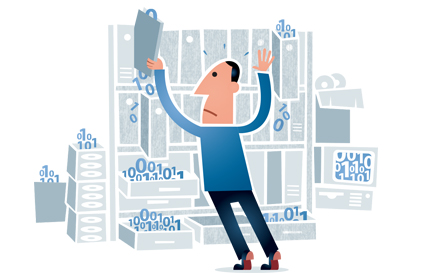
\includegraphics[width=.6\textwidth]{datamanagement-issues}
    
\includegraphics[width=.32\textwidth]{question}
\end{frame}

\begin{frame}
    \frametitle{Présentation du projet}
    \framesubtitle{Objectifs}
    \begin{columns}
        \begin{column}{0.5\textwidth}
            \begin{figure}
                
\includegraphics[width=1\textwidth]{logo-citywatch}
            \end{figure}
        \end{column}
        \begin{column}{0.5\textwidth}
            \begin{itemize}
                \item Startup
                \item 8 membres
                \item Services de consultings
                \item Informations routiers
            \end{itemize}
        \end{column}
    \end{columns}
\end{frame}

\begin{frame}
    \frametitle{Objectifs du projet}
    \begin{figure}
        \centering
        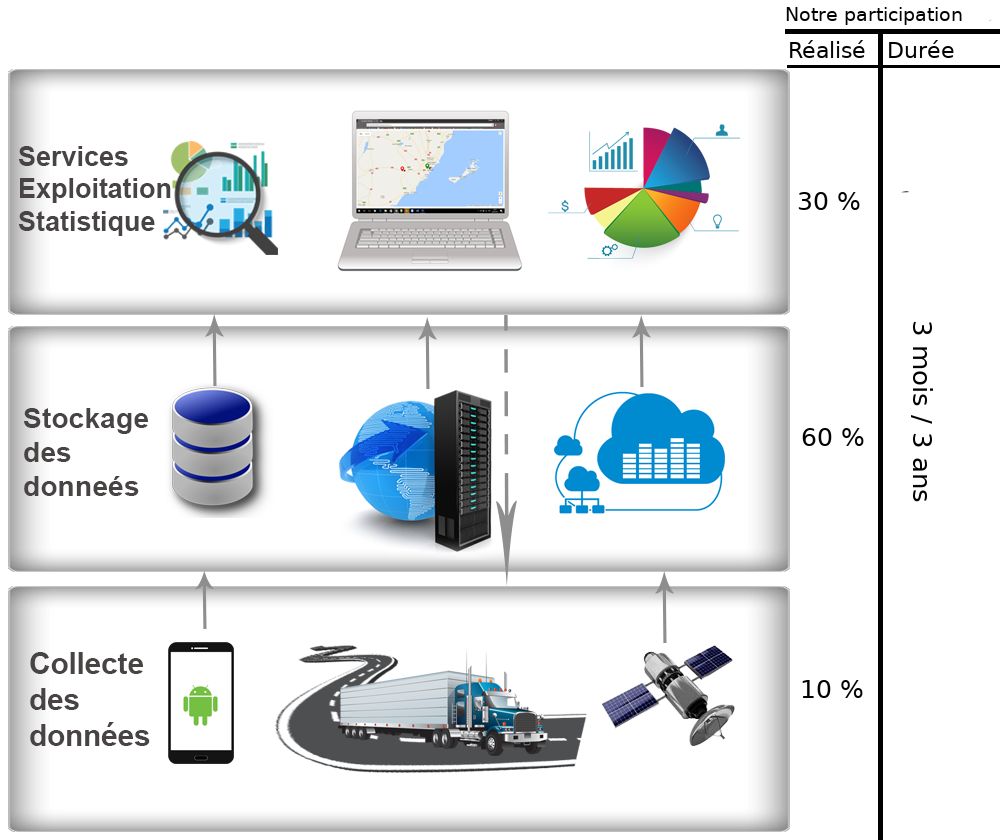
\includegraphics[width=.85\textwidth]{citywatch-modules-participation}
    \end{figure}
\end{frame}

\section{Gestion de projet selon SCRUM}

%\begin{frame}
%    \frametitle{Pourquoi SCRUM}
%    \centering
%    
\includegraphics[width=.7\textwidth]{scrum-logo}
%\end{frame}

\begin{frame}
    \frametitle{Méthode SCRUM}
    \centering
    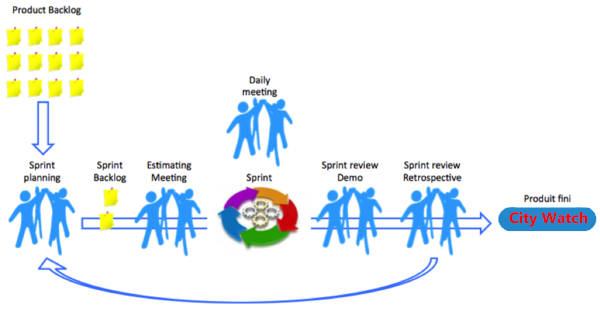
\includegraphics{scrum-model}
\end{frame}

\begin{frame}
\frametitle{Découpage du projet}
\begin{figure}
%    \smartdiagram[descriptive diagram]{%
%  {Itération 0, {Préparatifs à SCRUM}},
%  {Itération 1, {Service de localisation}},
%  {Itération 2, {Gestion des rapports}},
%  {Itération 3, {Service web d'authentification}}}
    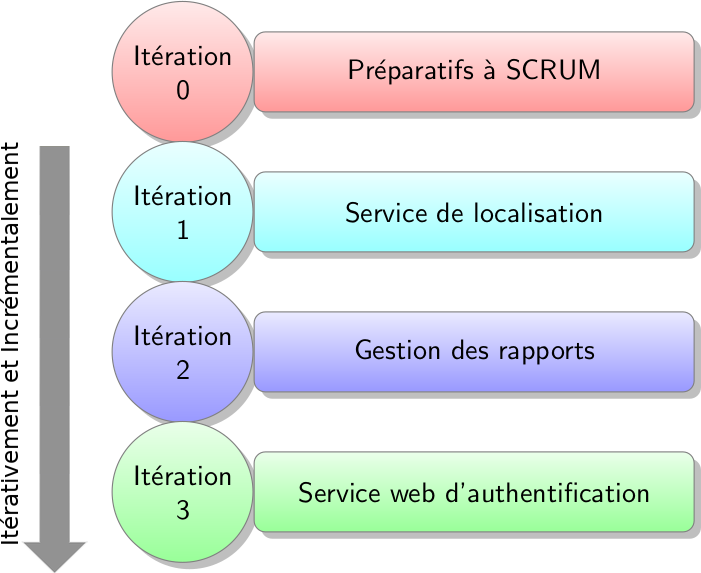
\includegraphics[width=.87\textwidth]{sprints-overview}
\end{figure}
\end{frame}

\section{Itération 1: Service Localisation}

\begin{frame}
    \frametitle{But de l'itération}
    \begin{itemize}
        \item backend:
        \begin{itemize}
        \item Service web de géolocalisation
        \end{itemize}
    \item frontend:
        \begin{itemize}
        \item Application mobile qui détecte la position géographique.
        \item Projection de positions sur une carte Google map.
    \end{itemize}
    \end{itemize}
\end{frame}

\begin{frame}
    \frametitle{Diagramme de cas d'utilisation}
    \begin{figure}
        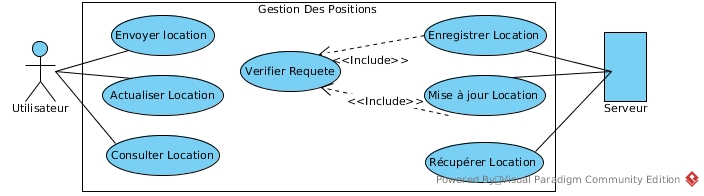
\includegraphics[width=1\textwidth]{sprint1-webservices-usecase}
    \end{figure}
\end{frame}

\begin{frame}
    \frametitle{Diagramme de séquences}
    \begin{figure}
        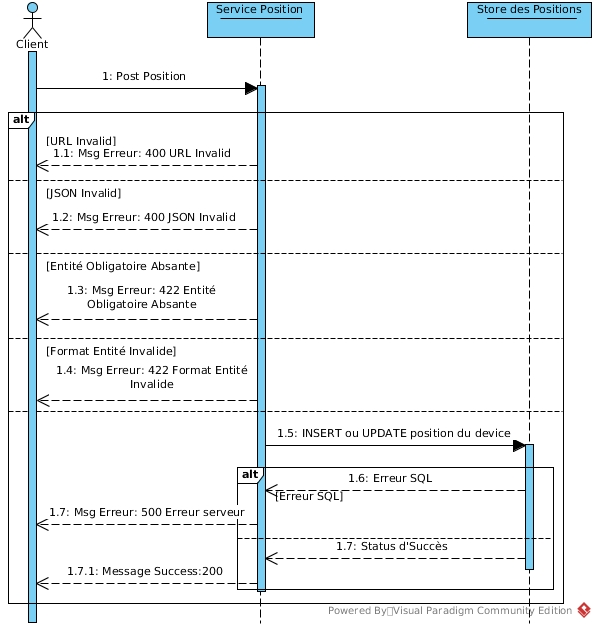
\includegraphics[width=0.7\textwidth]{sprint1-webservices-post-sequence}
    \end{figure}
\end{frame}

\begin{frame}
    \frametitle{Prototype de l'itération}
    \begin{figure}
        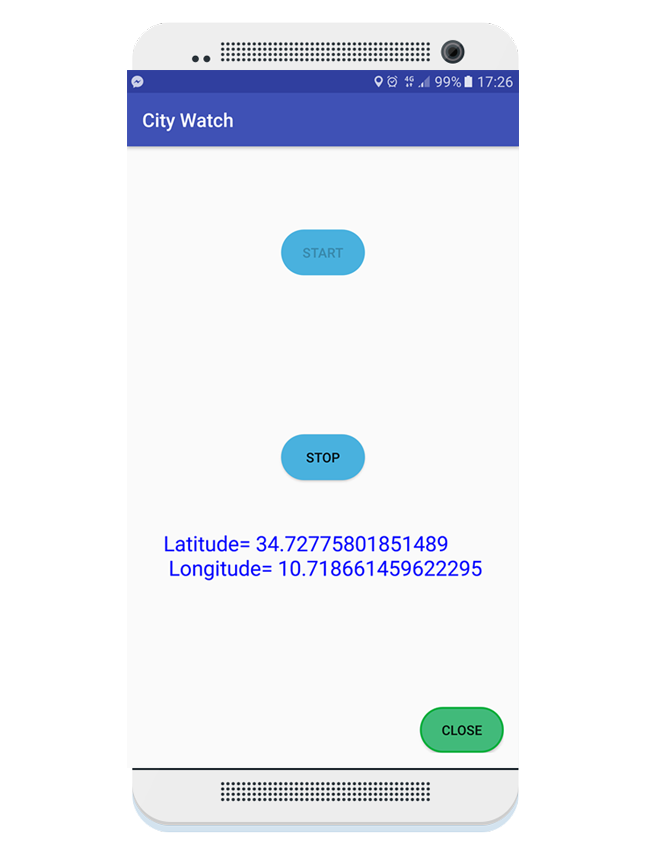
\includegraphics[width=0.3\textwidth]{sprint1-android-screenshot}
        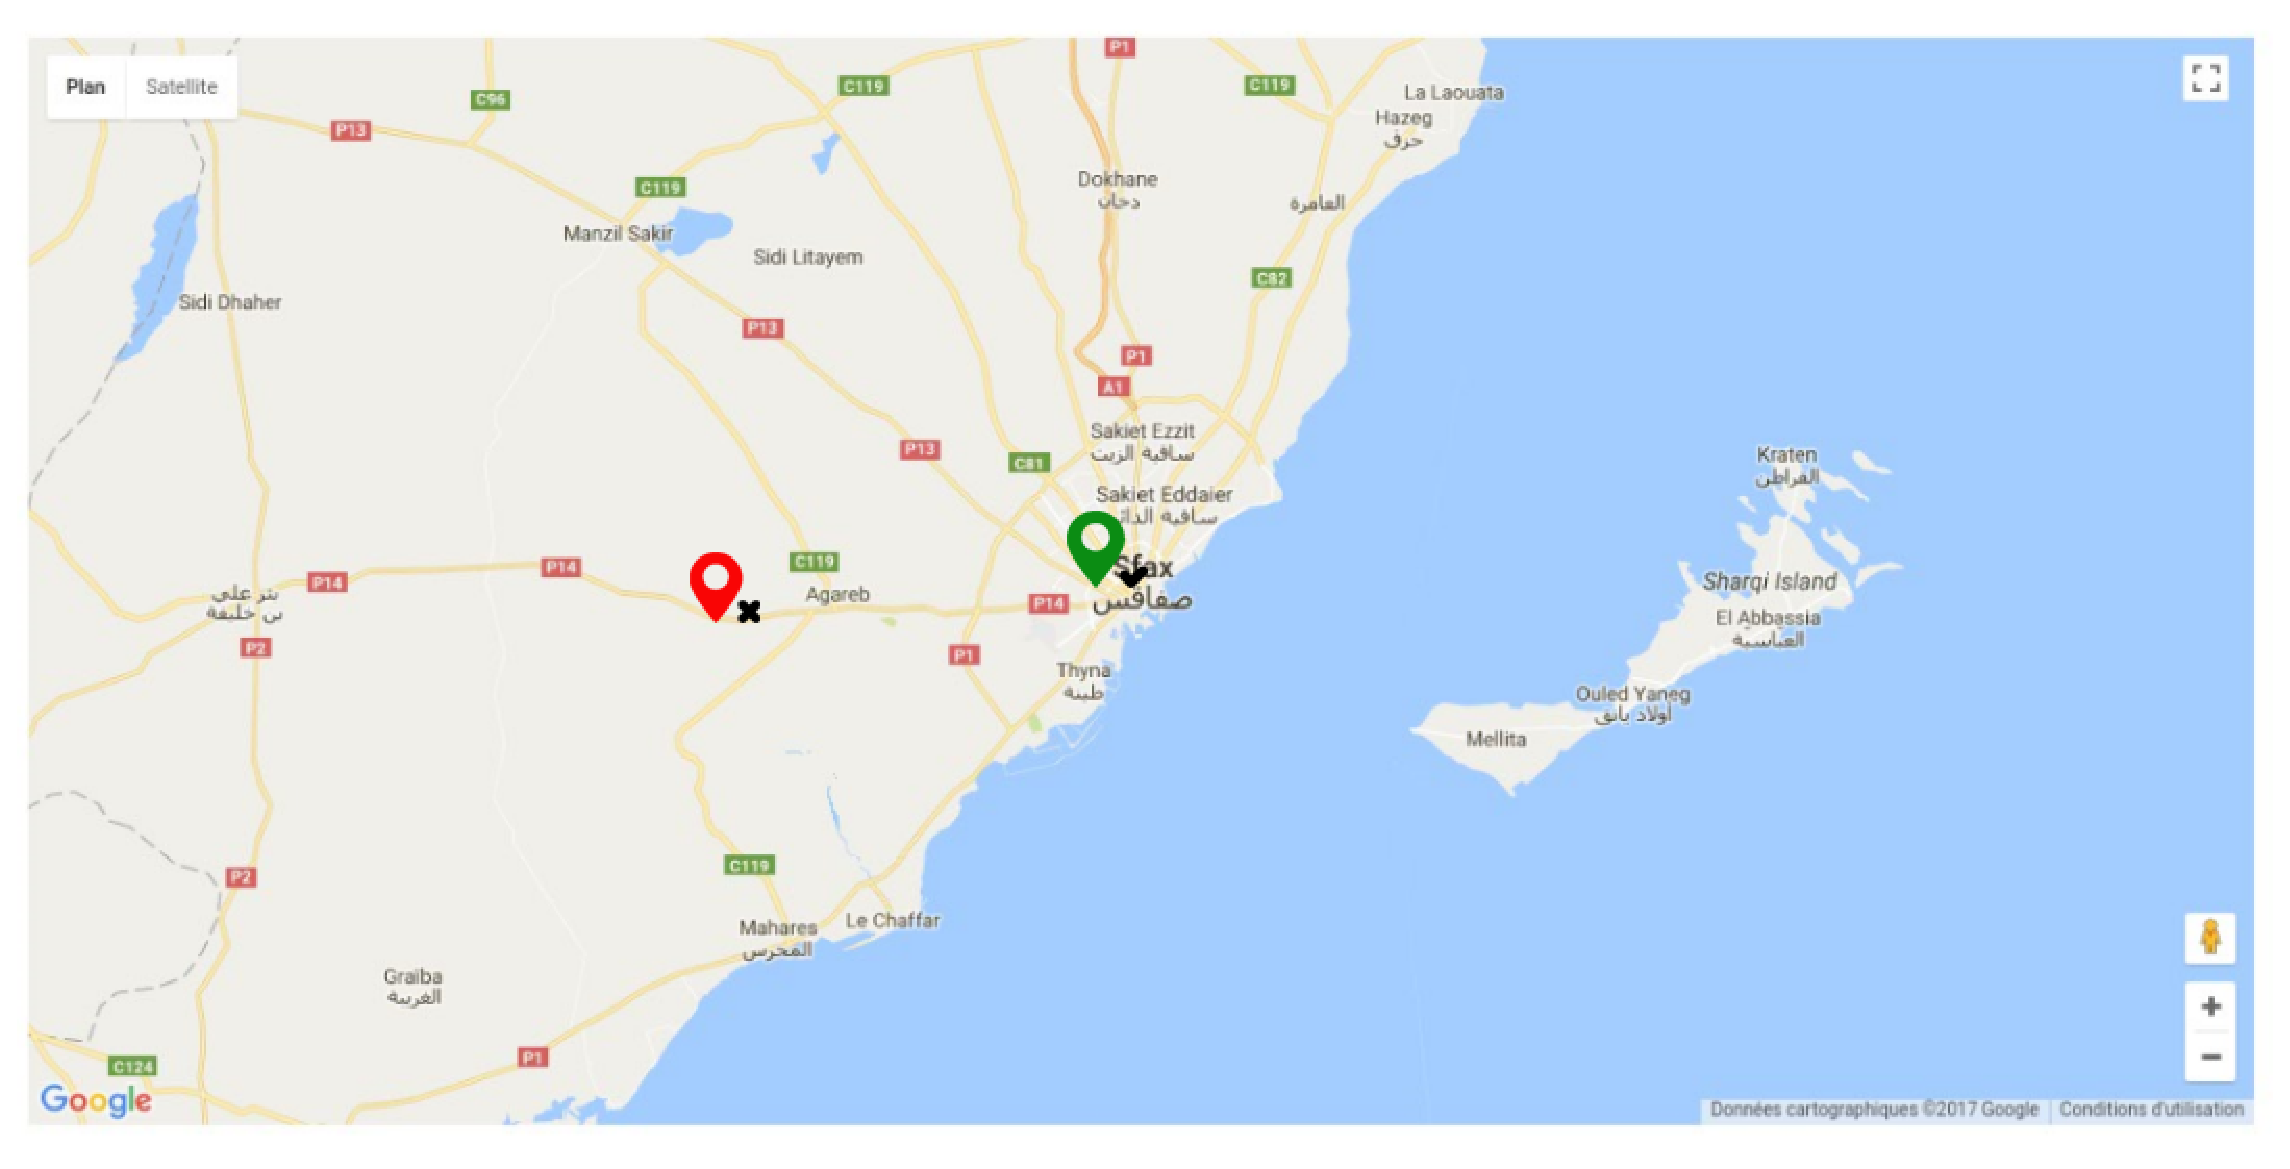
\includegraphics[width=0.7\textwidth]{sprint1-dashboard-screenshot}
    \end{figure}
\end{frame}

\begin{frame}
\frametitle{Évaluation de l'itération}
\begin{minipage}{\textwidth}
\usetikzlibrary{plotmarks}

\begin{figure}[H]
\centering
\begin{tikzpicture}[y=.2cm, x=.7cm,font=\sffamily]
\begin{axis}[
xlabel=$Jours$,
ylabel=$Heures\ restantes$,
grid=both,
grid style={line width=.1pt, draw=gray!10},
width=0.9\textwidth,
height=8cm,
%major grid style={line width=.2pt,draw=gray!50},
]
      \addplot[gray!40] plot coordinates {%
(0, 412)
(18, 0)
    };
      \addplot[gray!40] plot coordinates {%
(0, 140)
(18, 0)
    };

    \addplot[mark=*,red] plot coordinates {%
        (0, 412)
        (1, 405)
        (2, 385)
        (3, 365)
        (4, 340)
        (5, 322)
        (6, 306)
        (7, 270)
        (8, 235)
        (9, 193)
        (10, 165)
        (11, 137)
        (12, 110)
        (13, 80)
        (14, 50)
        (15, 21)
        (16, 0)
        (17, 0)
        (18, 0)
    };
    \addlegendentry{Temps réellement pris}

    \addplot[mark=*,cyan] plot coordinates {%
        (0, 140)
        (1, 132)
        (2, 126)
        (3, 108)
        (4, 90)
        (5, 79)
        (6, 70)
        (7, 61)
        (8, 55)
        (9, 47)
        (10, 39)
        (11, 30)
        (12, 21)
        (13, 15)
        (14, 8)
        (15, 1)
        (16, 2)
        (17, 2)
        (18, 2)
    };
    \addlegendentry{Temps pris par binôme}
\end{axis}
\end{tikzpicture}
\caption{Graphique d'avancement - Itération 1}
\label{fig:sprint1-burndown}
\end{figure}

\end{minipage}
\end{frame}

\section{Itération 2: Gestion des Rapports}

\begin{frame}
    \frametitle{But de l'itération}
    \begin{itemize}
        \item Déclaration des rapports.
        \item Détection des secousses et des ralentisseurs.
        \item Consultation des trajectoires, des rapports, des secousses et des ralentisseurs.
    \end{itemize}
\end{frame}

\begin{frame}
    \frametitle{Diagramme de cas d'utilisation}
    \begin{figure}
        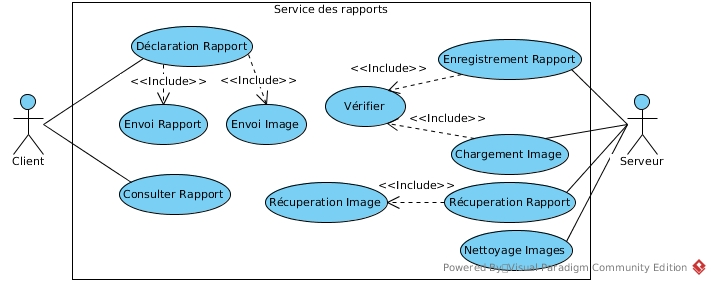
\includegraphics[width=\textwidth]{sprint2-webservices-report-usecase}
    \end{figure}
\end{frame}

\begin{frame}
    \frametitle{Diagramme de séquences}
    \begin{figure}
        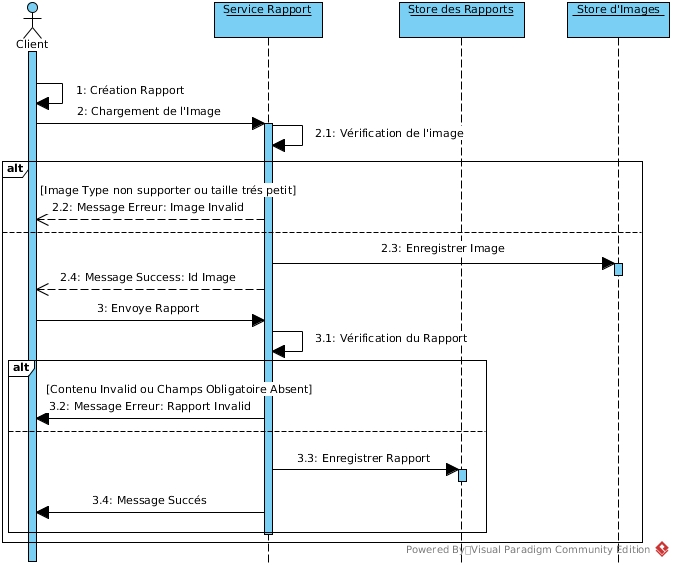
\includegraphics[width=.8\textwidth]{sprint2-webservices-report-post-sequence}
    \end{figure}
\end{frame}

\begin{frame}
    \frametitle{Prototype de l'itération}
    \begin{figure}
        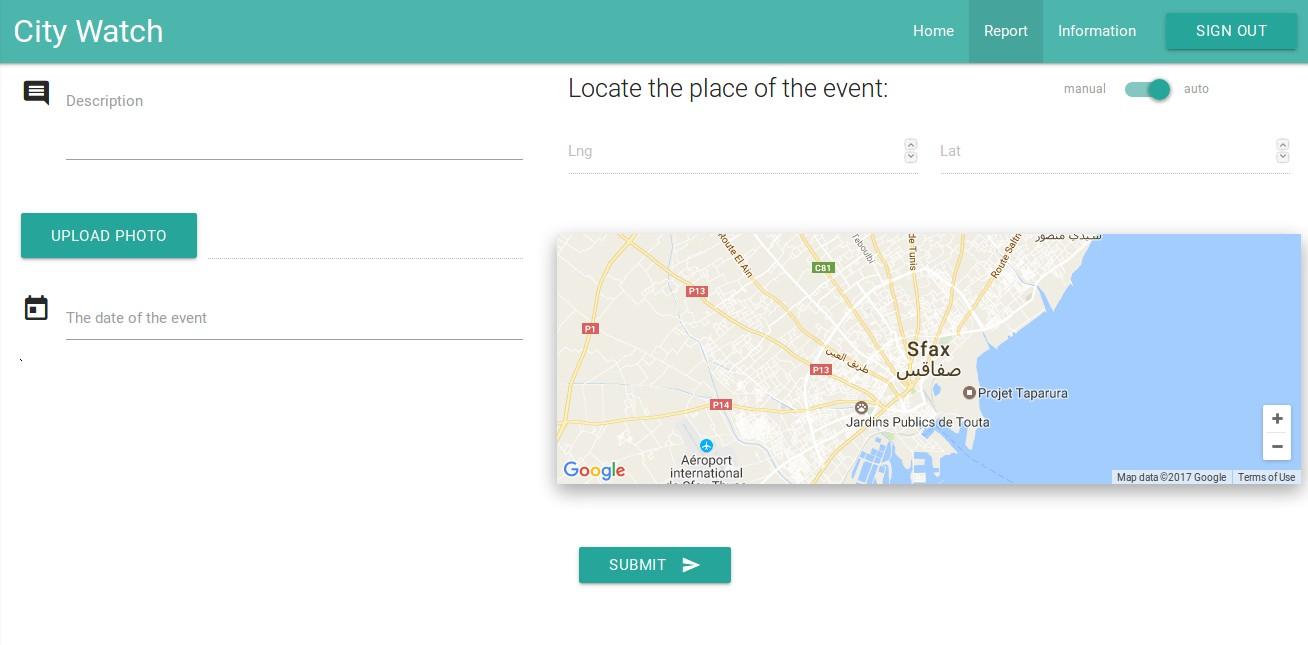
\includegraphics[width=0.45\textwidth,height=4cm]{sprint2-rapport-screenshot1}
        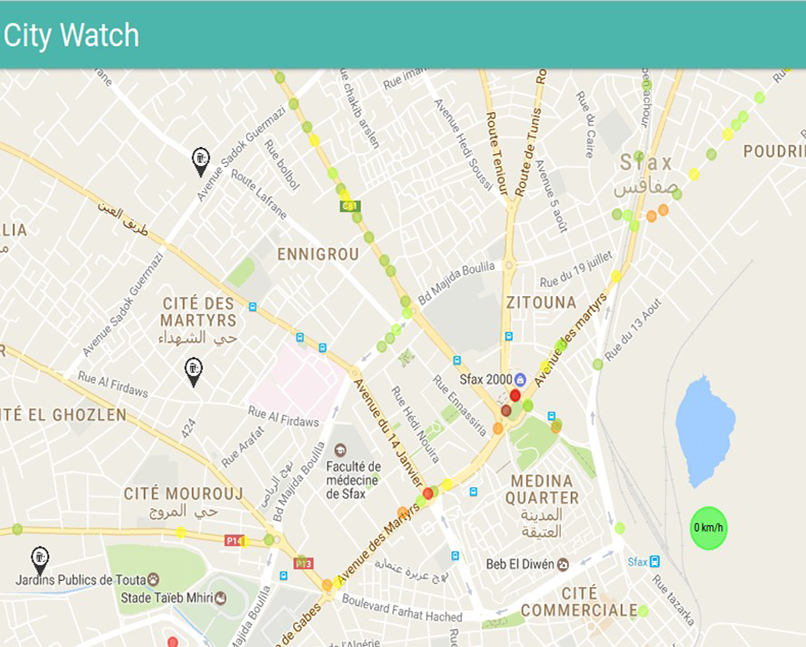
\includegraphics[width=0.5\textwidth]{sprint2-dashboard-screenshot2}
    \end{figure}
\end{frame}

\section{Itération 3: Service web d'authentification}

\begin{frame}
    \frametitle{But de l'itération}
    \begin{itemize}
        \item Détection et projection de la vitesse moyenne et de l'état du réseau cellulaire.
        \item Service web d'authentification
        \item Traitement et visualisation des données en procédant par ``Business Intelligence'': le cas des secousses.
    \end{itemize}
\end{frame}

\begin{frame}
    \frametitle{Diagramme de cas d'utilisation}
    \begin{figure}
        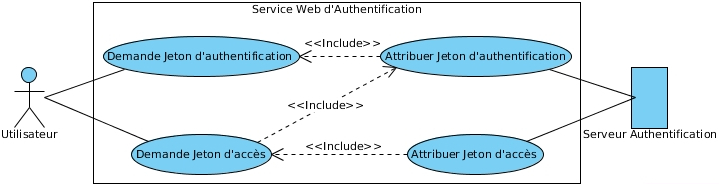
\includegraphics[width=\textwidth]{sprint3-webservices-oauth-usecase}
    \end{figure}
\end{frame}

\begin{frame}
    \frametitle{Diagramme de séquences}
    \begin{figure}
        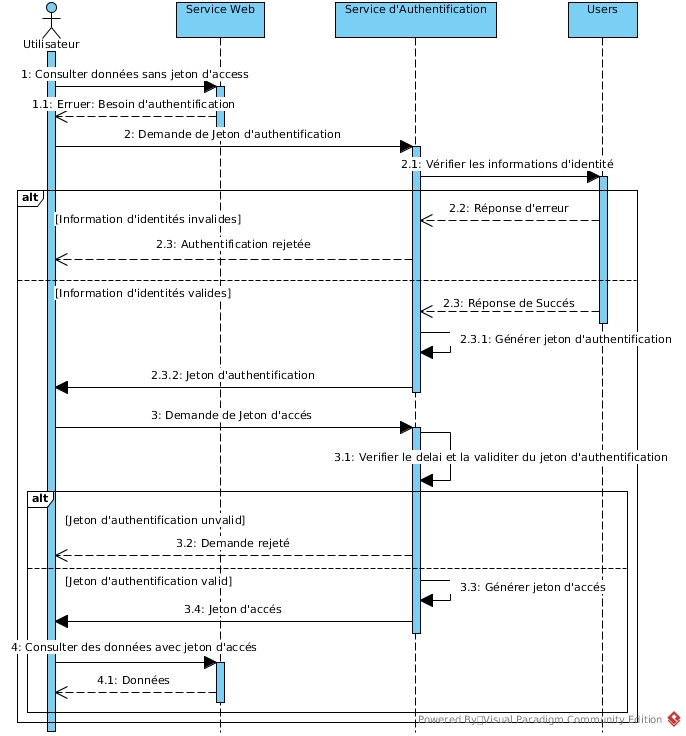
\includegraphics[width=.65\textwidth]{sprint3-webservices-oauth-sequence}
    \end{figure}
\end{frame}

\begin{frame}
    \frametitle{Prototype de l'itération}
    \begin{figure}
        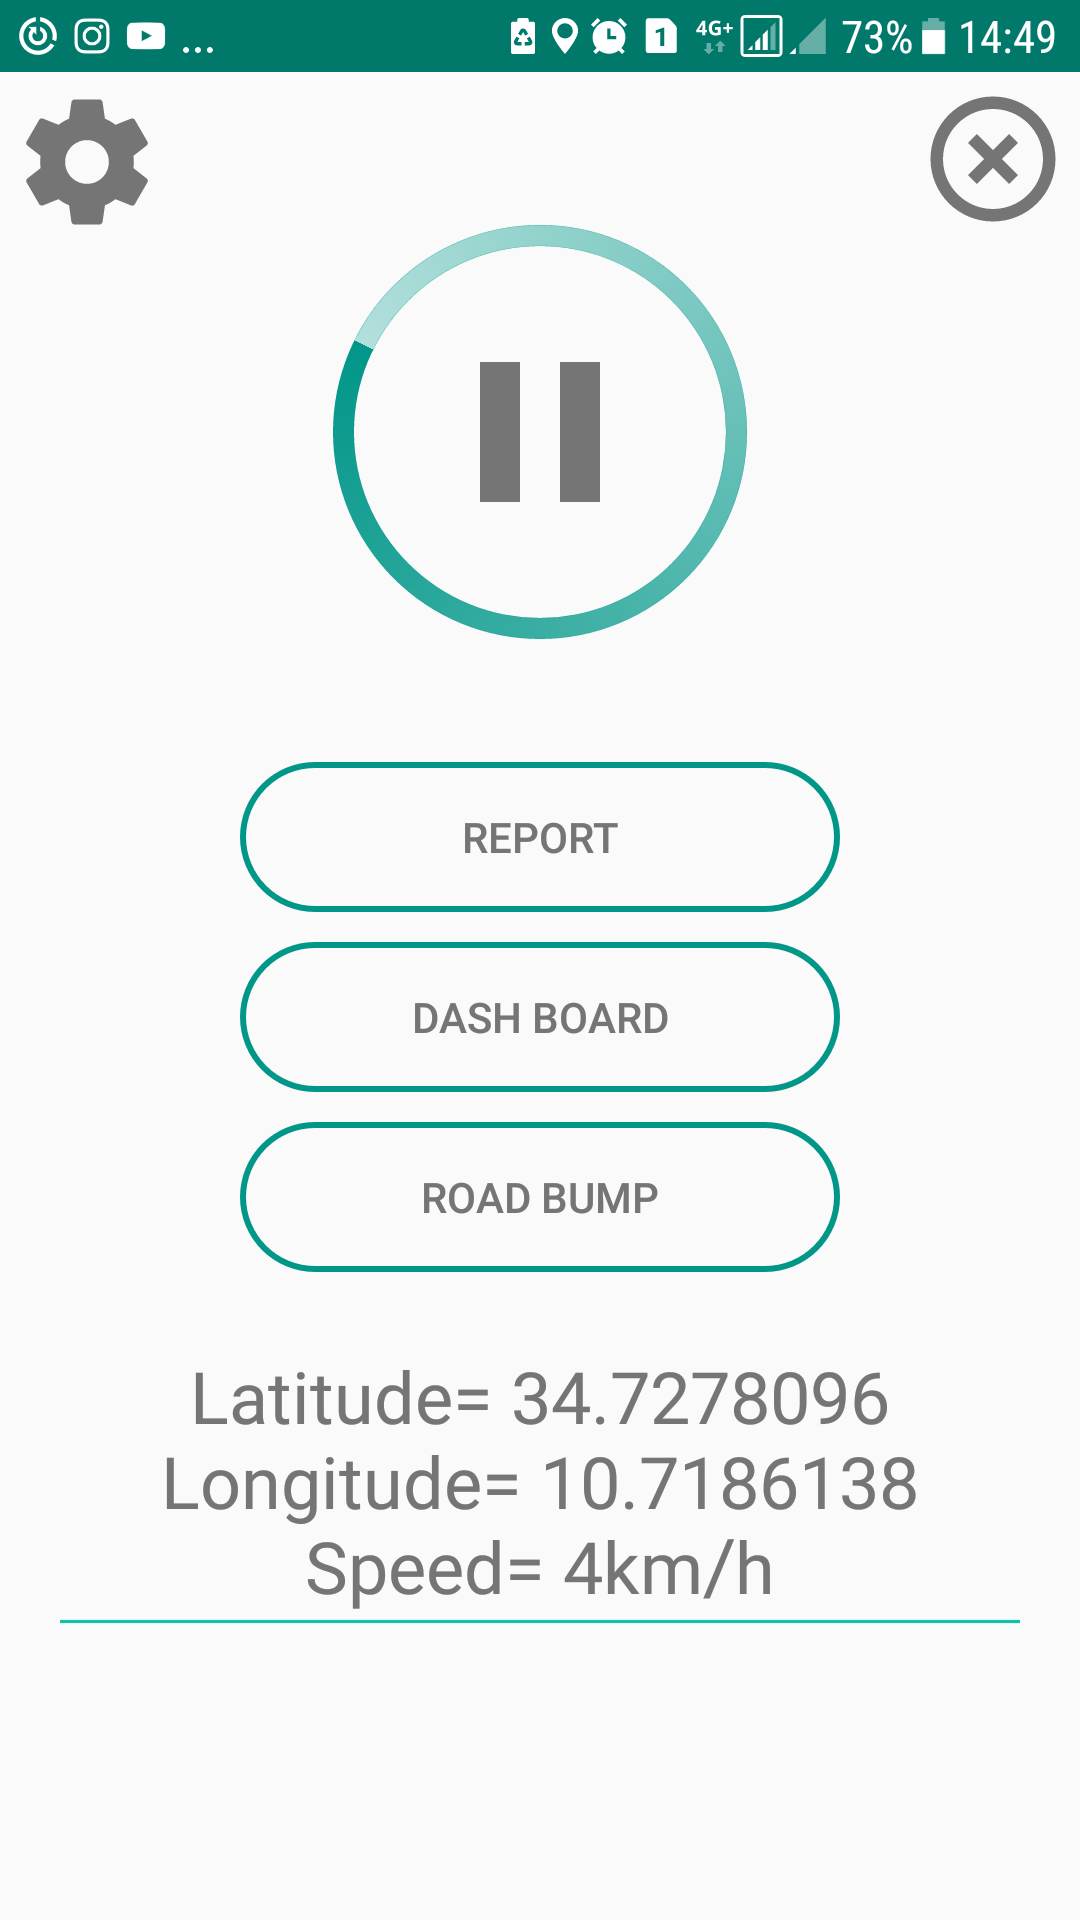
\includegraphics[width=0.35\textwidth]{sprint3-android-screenshot2}
        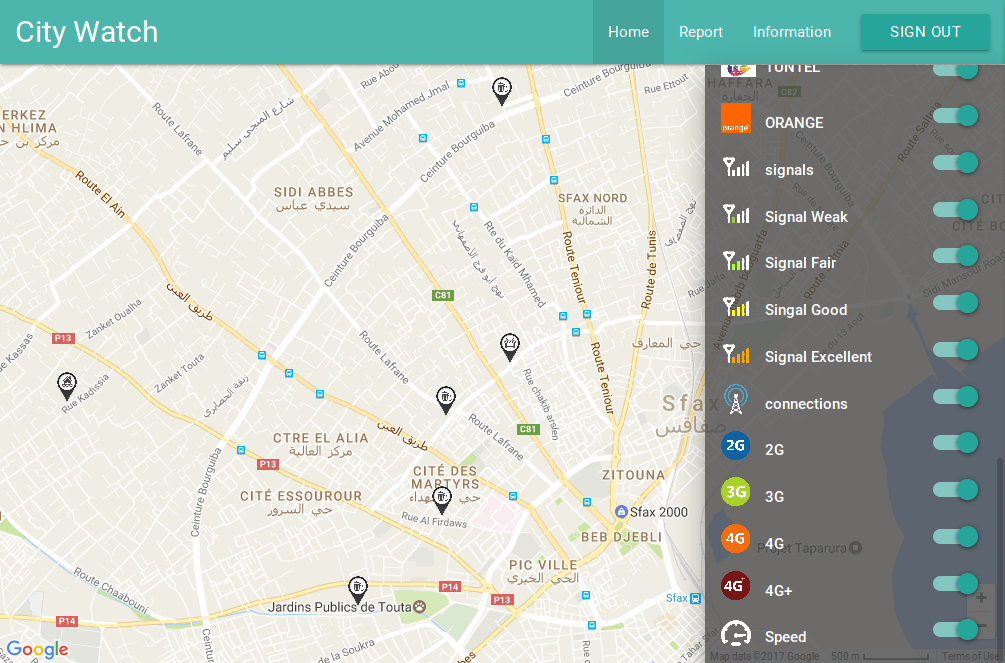
\includegraphics[width=0.67\textwidth]{sprint3-dashboard-screenshot1}
    \end{figure}
\end{frame}


\section{Réalisation}

\begin{frame}
    \frametitle{Technologies utilisées}
    \begin{description}
        \item [Architecture] \textbf{}

            \begin{itemize}
                \item MVC
                \item RESTful
            \end{itemize}
        \item [Langages de programmation] \textbf{}

            \begin{itemize}
                \item PHP 7
                \item JavaScript (ECMAScript 2016)
                \item Java
            \end{itemize}
        \item [Plateformes \& frameworks] \textbf{}

            \begin{itemize}
                \item Lumen
                \item Android
            \end{itemize}
    \end{description}
\end{frame}

\begin{frame}
    \begin{center}
    \begin{figure}
        
\includegraphics[width=0.9\textwidth]{demo}
    \end{figure}
    \end{center}
\end{frame}

\section{Conclusion \& Perspectives}

\begin{frame}
    \frametitle{Conclusion}
    \begin{itemize}
        \item Développer des Services Web tels que: service de géolocalisation et service de ralentisseurs.
        \item Gérer le projet suivant SCRUM: 3 itérations sont retenues.
        \item Maîtriser plusieurs technologies telles que JSON, RESTful, Android, OAuth2, etc.
        \item Améliorer nos compétences comportementales et managériales.
    \end{itemize}
\end{frame}

\begin{frame}
    \frametitle{Perspectives}
    \begin{itemize}
        \item Appliquer la solution dans des scénarios comme le calcul du chemin optimal suivant les caractéristiques des marchandises.
        \item Mettre en place tout le processus du Big Data.
        \item Implantation de la start-up ``City Watch''.
    \end{itemize}
\end{frame}

\begin{frame}
    \begin{center}
        \bfseries \Huge
        Merci
    \end{center}
\end{frame}

\section*{Annexe}
\begin{frame}
\frametitle{Diagrammes}
\textbf{TODO:} add class diagrams, database schema.
\end{frame}

\end{document}
